\documentclass{article}


\usepackage{arxiv}

\usepackage[utf8]{inputenc} % allow utf-8 input
\usepackage[T1]{fontenc}    % use 8-bit T1 fonts
\usepackage{hyperref}       % hyperlinks
\usepackage{url}            % simple URL typesetting
\usepackage{booktabs}       % professional-quality tables
\usepackage{amsfonts}       % blackboard math symbols
\usepackage{nicefrac}       % compact symbols for 1/2, etc.
\usepackage{microtype}      % microtypography
\usepackage{lipsum}
\usepackage{graphicx}

\title{Nested 3D neural networks for kidney and tumor segmentation}


\author{
  David S.~Hippocampus\thanks{Use footnote for providing further
    information about author (webpage, alternative
    address)---\emph{not} for acknowledging funding agencies.} \\
  Department of Computer Science\\
  Cranberry-Lemon University\\
  Pittsburgh, PA 15213 \\
  \texttt{hippo@cs.cranberry-lemon.edu} \\
  %% examples of more authors
   \And
 Elias D.~Striatum \\
  Department of Electrical Engineering\\
  Mount-Sheikh University\\
  Santa Narimana, Levand \\
  \texttt{stariate@ee.mount-sheikh.edu} \\
  %% \AND
  %% Coauthor \\
  %% Affiliation \\
  %% Address \\
  %% \texttt{email} \\
  %% \And
  %% Coauthor \\
  %% Affiliation \\
  %% Address \\
  %% \texttt{email} \\
  %% \And
  %% Coauthor \\
  %% Affiliation \\
  %% Address \\
  %% \texttt{email} \\
}

\begin{document}
\maketitle

\begin{abstract}
\lipsum[1]
\end{abstract}


% keywords can be removed
\keywords{First keyword \and Second keyword \and More}


\section{Introduction}
\label{sec:intro}
\section{Methodology}
\label{sec:methods}

\subsection{Preprocessing}
\label{sec:prepro}
The proprocessing steps performed are:
\begin{enumerate}
    \item Resample the image to a resolution of $2 \times 2 \times 2$ mm. 
    \item Crop a cube of size $168^3$ from the center of the image. 
    \item Normalize the intensities to a range of 0 to 1.
\end{enumerate}

\subsection{Neural Network Architecture}
\label{sec:nnarc}
The proposed method contains two NN with the same architecture, one is used to segment the kidneys and the other one 
is used to segment the tumors. 

Each NN is a 3D U-Net with 14 convolutional layers. Each convolutional layer has a relu function as activation and uses
filter sizes of $3\times 3 \times 3$. The input size is the preprocessed image with size $168^3$. 

\begin{figure}[h]
    \centering
    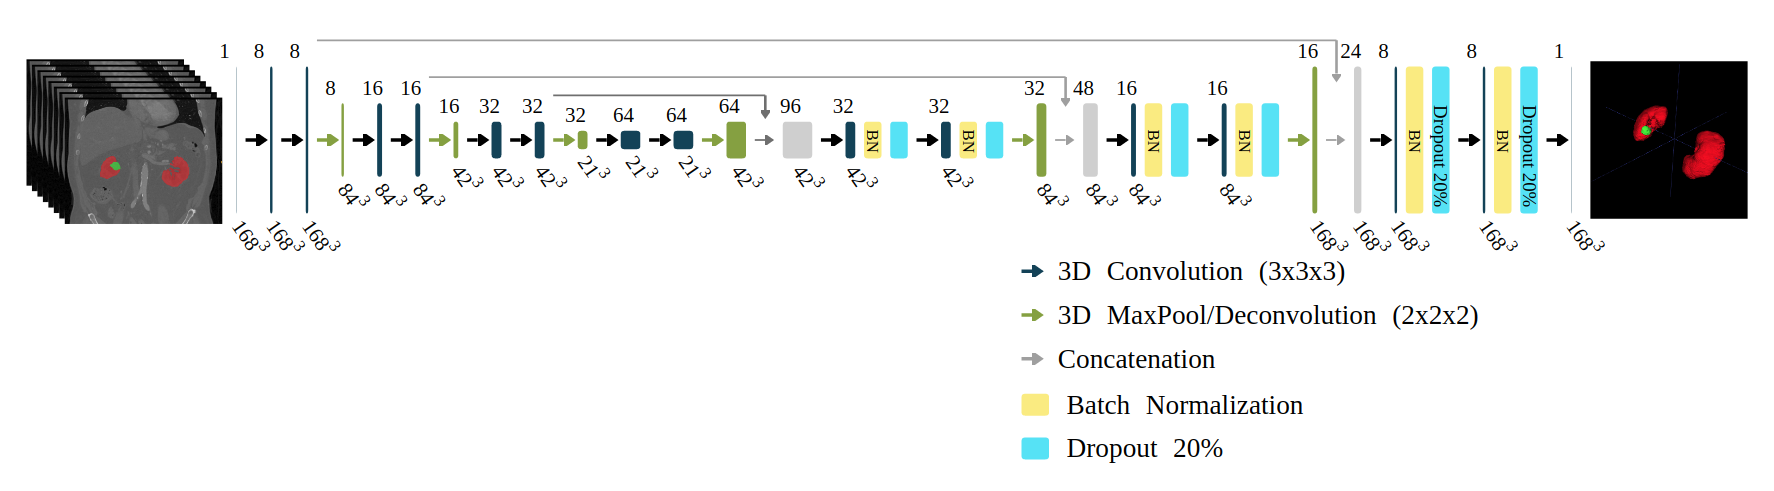
\includegraphics[totalheight=.20\textheight]{imgs/nn.png}
    \caption{NN architecture }
    \label{fig:mobile1}
\end{figure}


\end{document}
